\documentclass[a4paper]{report}

\usepackage[british]{babel}

\usepackage{listings}
\usepackage{color}

\usepackage{graphicx}
\graphicspath{ {./images/} }

\usepackage{wrapfig}

\definecolor{dkgreen}{rgb}{0,0.6,0}
\definecolor{gray}{rgb}{0.5,0.5,0.5}
\definecolor{mauve}{rgb}{0.58,0,0.82}

\lstset{frame=tb,
  language=C,
  aboveskip=3mm,
  belowskip=3mm,
  showstringspaces=false,
  columns=flexible,
  basicstyle={\small\ttfamily},
  numbers=none,
  numberstyle=\tiny\color{gray},
  keywordstyle=\color{blue},
  commentstyle=\color{dkgreen},
  stringstyle=\color{mauve},
  breaklines=true,
  breakatwhitespace=true,
  tabsize=4
}

\title{A Level Computer Science NEA}
\author{Bailey Harrison}
\date{
	\today\endgraf\bigskip
	Z80 Assembler
}

\begin{document}

\maketitle

\tableofcontents



\chapter{Analysis}

\section{Introduction}

An assembler is a computer program that translates low-level assembly
instructions into raw machine code and data. Unlike compilers and interpreters,
assemblers lack many of the high-level control statements that most programmers
are used to, such as 'if' statements and 'for' loops.

Generally, there is a 1:1 correspondence between assembler opcodes (an acronym
specifying the operation) and machine code instructions (the binary data that a
CPU decodes and executes). Assemblers also support a few other features, notably
labels. A label serves as a placeholder for a memory address, which can be used
to implement variables and functions in a program. In the case of my project, I
am writing an writing an assembler for the Z80 processor architecture.

\bigskip

\begin{wrapfigure}{l}{0.25\textwidth}
    \centering
    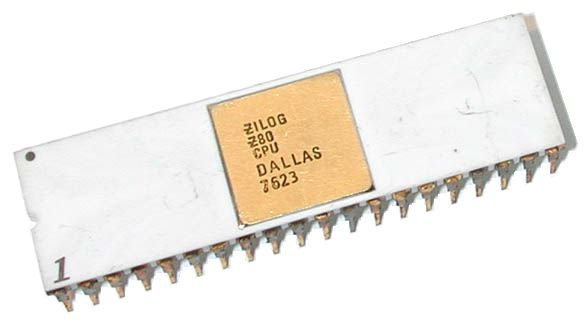
\includegraphics[width=0.25\textwidth]{z80}
\end{wrapfigure}

The Z80 CPU is a microprocessor invented by Zilog in 1975 as their first
product. It was designed as a largely software-compatible extension of the Intel
8080 CPU. Despite the Z80 being originally designed for use in embedded systems,
it gained massive popularity in the desktop market. The Z80 was used in
countless personal computers in the time period, such as the ZX 81, ZX Spectrum,
and Amstrad CPC. Many older game consoles also used this processor, notable the
Nintendo Gameboy and Sega Game Gear. In the modern day, the Zilog Z80 continues
to be used in Texas Instruments' line of TI-83/84 graphing calculators.

\section{Problem}

When programming for older computer systems, you have to take into account the
limited processing power and memory of these systems. Higher-level languages
have a performance overhead and their abstract nature prevents the programmer
from fully taking advantage of the available hardware. Even common "systems"
languages like C and C++ do not allow the programmer to have full control of
memory allocation, register usage, and what particular machine code instructions
are generated.

It is for this reason that retro computer programmers almost exclusively use an
assembly language for development. There is not just one clear-cut design for an
assembler, the level of complexity can vary greatly. For my target's needs, I
deemed it adequate to use one of the more simple assembler designs: a 2-pass
assembler.

\subsection{What is a 2-pass assembler?}

Unlike many programming languages, it is often the case than a program written
in assembly language will need to call/reference a label defined later on in the
program. If an assembler were to only read through the assembly source file
once, it would be impossible to resolve these forward label references. This is
because the assembler will have not yet encountered those label definitions, and
will therefore be unable to calculate the correct operand value in the outputted
machine code file.

To resolve this issue, an assembler can instead read through the source file
twice. During the first pass, all references to labels as operands can be
ignored. When a label definition is encountered, the assembler adds the
label name and its corresponding memory address to a symbol table.

During the second pass, if a label reference is encountered in an operand
argument, the symbol table is used to find the corresponding value. The value
can then be easily appended to the machine code file as the source file is being
read.

\section{System objectives / specification}

\begin{enumerate}

\subsection{Required}

	\item \label{req_inputFile}
		Allow the input file to be specified on the command line
	\item \label{req_doAsm}
		Implement the assembler in 2 passes: symbol table, and assembly
	\item \label{req_doLabels}
		Support labels in the code
	\item
		Calculate the offset for relative jumps from a label
	\item
		Allow integer literals to be specified in denary and hexadecimal
	\item
		Instruction set: support the main 256 Z80 instructions

\subsection{Optional}

	\item Instruction set: support extended instructions
	\item Instruction set: support ix/iy instructions
	\item Instruction set: support bit instructions
	\item Allow the output file to be specified
	\item Have an assembler directive that specifies the starting memory address
		(.org)
	\item Have assembler directives for placing arbitrary bytes into memory
		(.db, .dw)

\end{enumerate}



\chapter{Design}

\section{Getting command line arguments}

To begin this project, the first problem I decide to tackle is parsing command
line arguments. Once I get to the stage where a user can specify an input file
and possibly any options, that will set up a nice foundation on which the actual
assembler can be built.

To do this, I first test that the user has entered at least one command line
argument by testing the value of the \texttt{argc} variable, which is set
by the operating system when the program is run. This variables give the number
of command line arguments (including the name of the program itself), so I test
if the variable is 1 or less, and if so, print out some help text.

\begin{lstlisting}
// main.c
// line 30
if (argc <= 1) {
	usage(argv[0]);
	exit(EXIT_FAILURE);
}
\end{lstlisting}

The above referenced \texttt{usage()} function displays the help text, taking
the name of the called program as input.

\begin{lstlisting}
static void usage(char *argv0)
{
    fprintf(stderr, "usage: %s [-hv] [-o output_file] file\n", argv0);
}
\end{lstlisting}

In C, every command line argument is passed to \texttt{main()} as a member of an
array of strings: \texttt{argv}. So to access the first command line argument, I
would write \texttt{argv[1]}, as \texttt{argv[0]} would reference the program
name.

To parse the list of command line arguments, I use a \texttt{for} loop. The
loop iterates through every character in each member of \texttt{argv} and will
only proceed if the argument begins with a \texttt{'-'} character. As per the
usage string, every command line option must begin with a hyphen to indicate
that it is an option. Options can be combined into one argument or specified
seperately. For instance, \texttt{assembler -h -v} (to bring up the help menu
and display the version) could also be written as \texttt{assembler -hv}. When
an option is encountered, a \texttt{switch} statement executes the correct
branch of code to satisfy that option.

The very last argument will always be interpreted as the input file name, and
an error will be thrown if this file name is not provided.

The options I implement are help (\texttt{-h}), version (\texttt{-v}), and
output file (\texttt{-o [filename]}). The output file name is copied into the
variable \texttt{outfile\_name} which is initialised to \texttt{"out.bin"} if
this option is not used.

\begin{lstlisting}
	char outfile_name[64] = DEFAULT_OUTFILE_NAME;

	int o = 1; // the char index into the argument string
    int i;
    for (i = 1; *(argv[i]) == '-' && i < argc; o++) {
        switch (argv[i][o]){
        case 0:     // go to next argument
            o = 0;
            i++;
            break;
        case 'h':
            usage(argv[0]);
            exit(EXIT_SUCCESS);
        case 'v':
            version();
			exit(EXIT_SUCCESS);
		case 'o':
			if (argc < i + 3) die("No output filename provided");
			i++;
			strncpy(outfile_name, argv[i], 63);
			if (strlen(outfile_name) != strlen(argv[i])) {
				die("Output filename too long");
			}
			o = 0;
			i++;
			break;
        default:
			usage(argv[0]);
			exit(EXIT_FAILURE);
        }
        if (i == argc) die("No input filename provided");

    }

	if (argc > i + 1) die("Multiple files specified");
\end{lstlisting}

\section{Pass 1: symbol table}

Now that the input file and output file names have been retrieved, I can proceed
to implement the first pass of the assembler: the symbol table.

Because the number of symbols defined in a source file is unknown, I decide to
use a linked list to store the symbol table entries. Linked lists allow for the
size of the list to change dynamically, and no memory will be wasted if the
list ends up being smaller than the allocated size. If I weren't to use a linked
list, I would either have to do another pass to find the number of labels, or I
would have to allocate a list of an arbitrarily large size. The former
alternative isn't ideal as an extra pass would cause the program to no longer be
a `2-pass assembler'. The latter alternative is unsuitable because if the user
defines too many symbols, the assembler will be unable to assemble the code.

I define each element of the linked list as a structure that holds the symbol
name, symbol value, and a pointer to the next element in the list. I then declare
the functions used to access and modify the symbol table.

\begin{lstlisting}
struct symbol {
	const char *label;
	int value;
	struct symbol *next;
};

size_t symtable_len(const struct symbol *symtable_head);
int symtable_search(const struct symbol *symtable_head, const char *label);
size_t symtable_build(FILE *fp, struct symbol **symtable_head);
void symtable_print(struct symbol *symtable_head);
\end{lstlisting}

\texttt{symtable\_len()} is a simple function that loops through every symbol
entry's \texttt{next} pointer until it encounters the end of the list. The
number of iterations is the returned length of the list.

\texttt{symtable\_search()} perfoms a linear search on the list, returning the
value which corresponds to the specified label name;

\bigbreak

Of the four functions just declared, \texttt{symtable\_build()} is the most
important, as it is the function that does the entire first pass of the
assembler.

This function works by looping through every line of the source file, important
information from the line, such as if any labels are defined, as well as any
opcode or operands are retrieved via the \texttt{parseline()} function. This
function returns its data in a structure which is layed out as follows:

\begin{lstlisting}
struct line_data {
	
	char *new_label; // empty if no label is defined

	ssize_t opcode_sz; // if 0, no opcode
	uint8_t opcode[3]; // start at [0]
	enum OpcodesPseudo pseudo_op; // use if opcode_sz == -1

	size_t operand_sz; // if 0, no operand
	char operand_label[LABEL_MAX_LEN+1]; // when empty, use operand_literal instead
	uint16_t operand_literal; // little endian
};
\end{lstlisting}

This function is not yet implemented at this stage, but it can be treated as a
black box which returns all vital information from the current line.

For the first pass, the only returned piece of information that's important is
the \texttt{new\_label} member, which, if not equal to \texttt{NULL} will
contain the name of a newly defined label.

If a new label is defined, I add the symbol to the linked list by allocating
memory for a new entry using \texttt{calloc()} and set the entry's \texttt{next}
pointer to the current head of the linked list. I then make this entry the
head of the linked list.

\begin{lstlisting}
	if (data.new_label != NULL) {
		struct symbol *new_symbol = calloc(sizeof(struct symbol), 1);
		new_symbol->label = data.new_label;
		new_symbol->value = address;
		new_symbol->next = *symtable_head;
		*symtable_head = new_symbol;
	}
\end{lstlisting}

Since the purpose of the first pass is to build a list of symbol names which are
mapped to memory addresses, the first pass will have to check if a line contains
the \texttt{.org} pseudo-instruction. This instruction changes the current
memory address of assembled code proceeding it. Therefore, any label definitions
after a \texttt{.org} pseudo-instruction will have to take this into account.

After checking if the current line contains a label definition, I check if the
current line contains a \texttt{.org} call. If it does, I change the current
assembly address to the argument of \texttt{.org}. To support
pseudo-instructions, I test for a special case where the opcode size is
\texttt{-1}. This indicates that the current opcode is in fact a pseudo-opcode.

\begin{lstlisting}
if (data.opcode_sz == -1 && data.pseudo_op == PSEUDO_ORG) {
	if (data.new_label != NULL) die("Cannot define label on same line as .ORG");
	if (data.operand_label[0] != '\0') {
		die("ERROR on line %d: .ORG cannot use labels\n", line_no);
	}
	address = data.operand_literal;
}
\end{lstlisting}

At the end of every iteration, I increment the current assembly address by the
size of the current instrution in bytes.

\begin{lstlisting}
address += line_assembled_size;
\end{lstlisting}

\section{Pass 2: assembly}

Now that the symbol table has been built, it is possible to pass through the
file only once more. I wrap this entire second pass in the \texttt{assemble()}
function, which takes the currently open file, the symbol table, and the output
memory buffer as arguments.

\begin{lstlisting}
void assemble(FILE *fp, const struct symbol *symtable_head, char *memory);
\end{lstlisting}

Just like the \texttt{symtable\_build()} function used to perform the first
pass, a \texttt{while} loop is used to pass through the file, and the
\texttt{parseline()} function is used to get important data from the line.

After retrieving the opcode, operands, and any label definitions on the line
(all returned from \texttt{parseline()}), I first test if the opcode size is
greater than \texttt{0}, as \texttt{0} means that there is no instruction on the
line, and \texttt{-1} means that the instruction on the line is a
pseudo-instruction.

Every byte of the opcode is then copied into the output buffer, proceeded by the
operand. However, if the current operand is a label reference, the symbol table
is checked to retrieve the correct value in place of this label name.

\begin{lstlisting}
if (data.opcode_sz > 0) {
	// copy opcode
	for (unsigned int i = 0; i < data.opcode_sz; i++) {
		memory[memindex++] = data.opcode[i];
	}

	// get operand
	uint16_t operand;
	if (data.operand_label[0] != '\0') {
		int symbol_value = symtable_search(symtable_head, data.operand_label);
		if (symbol_value == -1) {
			die("undefined label %s on line %d\n", data.operand_label, line_no);
		}
		operand = (unsigned)symbol_value & 0xFFFF;
	} else {
		operand = data.operand_literal;
	}

	// copy operand
	for (unsigned int i = 0; i < data.operand_sz; i++) {
		memory[memindex++] = (operand >> (i * 8)) & 0xFF;
	}
\end{lstlisting}

Just like in the first pass, I again test for the \texttt{.org}
pseudo-instruction and modify the current memory address accordingly. The reason
that I need to keep track of the current assembly address in the second pass is
because the Z80 has a few relative jump instructions. These instructions take as
an operand a twos-complement integer which represents the value which must be
added to the program counter to reach the referenced label. This is implemented
by simply subtracting the label address from the current address.

\begin{lstlisting}
// compute offset if instruction is relative jump
if (	data.opcode_sz == 1			&&
	   (data.opcode[0] == JR_N		||
		data.opcode[0] == JR_NZ_N	||
		data.opcode[0] == JR_Z_N	||
		data.opcode[0] == JR_NC_N	||
		data.opcode[0] == JR_C_N	||
		data.opcode[0] == DJNZ_N)	) {
	signed int offset = (signed int)operand - (signed int)address - 2;
	if (offset > 127 || offset < -128) {
		die("relative jump too far");
	}
	operand = (int8_t)offset;
}
\end{lstlisting}

Just as in the first pass, the current address is again incremented by the size
of the parsed instruction.

This is the end of the second pass.

\begin{lstlisting}
address += line_assembled_size;
\end{lstlisting}

Back in \texttt{main()}, the new \texttt{assemble()} function is called after
allocating space for the output file and rewinding the file pointer so that it
points to the beginning of the source file.

\begin{lstlisting}
// SECOND PASS
char* memory = calloc(memory_size, 1);
if (memory == NULL) die("Failed calloc()");
rewind(fp);
assemble(fp, symtable_head, memory);
fclose(fp);
\end{lstlisting}

\section{Parsing a line of assembly}

Now that the foundations of the assembler have been constructed, the main part
of the program that is missing is the \texttt{parseline()} function. Which until
now, has been left as a black box which does the neccesary processing to return
useful information from any given line of Z80 assembly.

There are 3 seperate pieces of data that must be retrieved from a line of
assembly. These are: the opcode (in machine code), the operand (whether a
literal or a label reference), and the name of the label defined on that line.
All of these fields are optional. A line may only contain an opcode and a line
may only contain a label definition, for instance. The only exception to this
rule is that a line must contain an opcode if there is also an operand.

To start off with, the first column of the line is checked to see if it is the
start of a comment (indicated by the semicolon character). If this is the case,
the function can safely return, having not found any instruction or label
definition.

\begin{lstlisting}
data->new_label = NULL;
data->opcode_sz = 0;
data->operand_sz = 0;
data->operand_label[0] = '\0';

if (line[0] == ';') return 0;
\end{lstlisting}

\subsection{Label definitions}

As a rule of my assembly language syntax, all label definitions must begin from
the first column of the line. They can only contain alphanumeric characters and
underscores but the first character cannot be numeric.

I check for this by looping through character-by-character, testing for many
conditions in the process. First, if the character is a semicolon, if it is,
the loop will exit as this is a comment. Second, I check if the current
character would be a valid label character. If it is, the current character will
be appended to the label name. If it is not, I check that the character is
either a tab, space, new line, or colon. As these are the only characters which
can appear after a label definition. If any of these characters are encountered,
the loop is ended.

\begin{lstlisting}
int len = 0;
for ( ;; ) { // infinite loop
	if (line[len] == ';')  break;
	int char_type = is_label_char_valid(line[len]);
	if (char_type == 1) len++;
	if (char_type == 0) {
		if (	line[len] != '\t' &&
				line[len] != '\n' &&
				line[len] != ' ' &&
				line[len] != ':') {
			die("line %d: Label contains an invalid character\n", line_no);
		} else {
			break;
		}
	}
}
\end{lstlisting}

The label is copied over and converted to lowercase as this assembler is not
case-sensitive. \texttt{malloc()} is used to allocate memory for this label

\begin{lstlisting}
data->new_label = malloc(len + 1);
for (int i = 0; i < len; i++) {
	data->new_label[i] = tolower(line[i]);
}
data->new_label[len] = '\0'; // add terminating 0
\end{lstlisting}

If a colon was specified after the label, it is then skipped over:

\begin{lstlisting}
if (line[index] == ':') {
	index++;
}
\end{lstlisting}

\subsection{Getting the opcode}

After a label definition, there must be tabs or spaces seperating it from the
opcode. I skip over them with a \texttt{for} loop.

\begin{lstlisting}
for ( ; line[index] == '\t' || line[index] == ' '; index++) ;
\end{lstlisting}

The opcode is copied over in a similar way to the label definition. The line
is looped through from the end of the label definition until a tab, space,
new line, or comment is encountered. Every character is checked to see if it
would be valid in an opcode using the \texttt{opcode\_char\_valid()} function.

The index variable is the same one used previously, so its current position will
be after the label definition and any whitespace following it.

\begin{lstlisting}
int len = 0; // length of opcode name
char opcode_name[OPCODE_NAME_MAX_LEN + 1] = { 0 };
for ( ;; ) { // infinite loop
	if (line[index] == ';') break;
	int char_valid = is_opcode_char_valid(line[index]);
	if (char_valid == 1) {
		// char is valid
		opcode_name[len] = line[index];
		len++;
		index++;
		if (len > OPCODE_NAME_MAX_LEN) {
			die("line %d: Opcode name too long\n", line_no);
		}
	} else {
		// char is not valid or is end of opcode
		if (	line[index] != '\n' &&
			line[index] != '\t' &&
			line[index] != ' '	) {
			die("line %d: Opcode contains invalid characters, char: %c\n", line_no, line[index]);
			exit(EXIT_FAILURE);
		} else break;
	}
}
if (strlen(opcode_name) == 0) return 0;
\end{lstlisting}

The \texttt{is\_opcode\_char\_valid()} function just checks each character and
only allows letters or a full-stop (for pseudo instructions).

\begin{lstlisting}
if (isalpha(c)) return true;
if (c == '.') return true;
else return false;
\end{lstlisting}

The name of the opcode is now stored in the \texttt{opcode\_name} variable.

\subsection{Getting the operands}

In my assembler's syntax, operands are specified as either numbers, labels, or
a register, any of which may also be surrounded by brackets. For example,
\texttt{(hl)}, \texttt{0x33}, and \texttt{myLabel} would be valid operands.

If there are multiple operands, they will all be saved into the same string at
this stage, their actual values will be parsed later.

To copy the operands string, I loop through the rest of the line until
encountering either a new line or a comment. Similar to what I did with the
opcode, I use the \texttt{is\_operand\_char\_valid()} function to avoid parsing
any invalid characters later on.

\begin{lstlisting}
int operand_str_size = 0;
char *start_of_operand = line + index;
for ( ;; ) {
	if (line[index] == ';') break;
	int char_valid = is_operand_char_valid(line[index]);
	if (char_valid == 1) {
		operand_str_size++;
		index++;
	}
	if (char_valid == 0) {
		if (line[index] != '\n') {
			die("ERROR: line %d: operand contains invalid character: %2X (hex)\n", line_no, line[index]);
		} else break;
	}
}
char *operand_str = NULL;
if (operand_str_size != 0) {
	operand_str = malloc(operand_str_size + 1);
	memcpy(operand_str, start_of_operand, operand_str_size);
	operand_str[operand_str_size] = 0; // null terminator
}
\end{lstlisting}

The \texttt{is\_operand\_char\_valid()} function serves as a simple filter that
rejects operands that are definitely invalid:

\begin{lstlisting}
if (isalnum(c)) return true;
switch (c) {
case ' ':
case '+':
case '-':
case '_':
case '(':
case ')':
case ',':
case '\'':
case '\t':
		return true;
default:
		return false;
}
\end{lstlisting}

\subsection{Finding the instruction}

Now that the opcode and operand strings have been retrieved, they are passed
into the \texttt{instruction\_lookup()} function which stores the operand's
machine code value and converted operands into a custom data structure.

\begin{lstlisting}
// figure out what the instruction is
instruction_lookup(opcode_name, operand_str, data);
\end{lstlisting}

The now-modified \texttt{data} variable is returned by the \texttt{parseline()}
function. This variable now contains the name of any newly defined label, the
correct binary opcode, and any converted operands.



%-------------------------------------------------------------------------------

\chapter{Technical Solution}

\section{Source files}

\lstset{numbers=left}

\subsection{main.c}
\lstinputlisting{../src/main.c}
\subsection{symtable.c}
\lstinputlisting{../src/symtable.c}
\subsection{assemble.c}
\lstinputlisting{../src/assemble.c}
\subsection{parseline.c}
\lstinputlisting{../src/parseline.c}
\subsection{util.c}
\lstinputlisting{../src/util.c}

\section{Header files}

\subsection{symtable.h}
\lstinputlisting{../src/symtable.h}
\subsection{assemble.h}
\lstinputlisting{../src/assemble.h}
\subsection{parseline.h}
\lstinputlisting{../src/parseline.h}
\subsection{util.h}
\lstinputlisting{../src/util.h}



\chapter{Testing}



\chapter{Appraisal}



\end{document}
